\documentclass[12pt]{article}
\usepackage{xcolor}
\usepackage[latin]{babel}
\usepackage[utf8]{inputenc}
\usepackage[T1]{fontenc}
\usepackage{amsmath}
\usepackage{amsfonts}
\usepackage{amssymb}
\usepackage[version=4]{mhchem}
\usepackage{stmaryrd}
\linespread{1.5}
\setlength{\parindent}{0pt}
\usepackage{listings}
\usepackage{xcolor}
\usepackage{algpseudocode}
\usepackage{tikz}
\usepackage{pifont}
\usepackage{tikz}
\usetikzlibrary{arrows.meta}
\usetikzlibrary{positioning}
\definecolor{mytextcolor}{rgb}{1,1,1}

\begin{document}

$\text{Q}_{1}$

1.{\small\textcircled{\scriptsize{2}}}$\rightarrow${\small\textcircled{\scriptsize{1}}}$\rightarrow${\small\textcircled{\scriptsize{4}}}$\rightarrow${\small\textcircled{\scriptsize{3}}}$\rightarrow${\small\textcircled{\scriptsize{6}}}$\rightarrow${\small\textcircled{\scriptsize{5}}}$\rightarrow${\small\textcircled{\scriptsize{8}}}$\rightarrow${\small\textcircled{\scriptsize{7}}}$\rightarrow${\small\textcircled{\scriptsize{14}}}$\rightarrow${\small\textcircled{\scriptsize{13}}}$\rightarrow${\small\textcircled{\scriptsize{16}}}$\rightarrow${\small\textcircled{\scriptsize{15}}}$\rightarrow${\small\textcircled{\scriptsize{10}}}$\rightarrow${\small\textcircled{\scriptsize{9}}}$\rightarrow${\small\textcircled{\scriptsize{12}}}$\rightarrow${\small\textcircled{\scriptsize{11}}}

2.


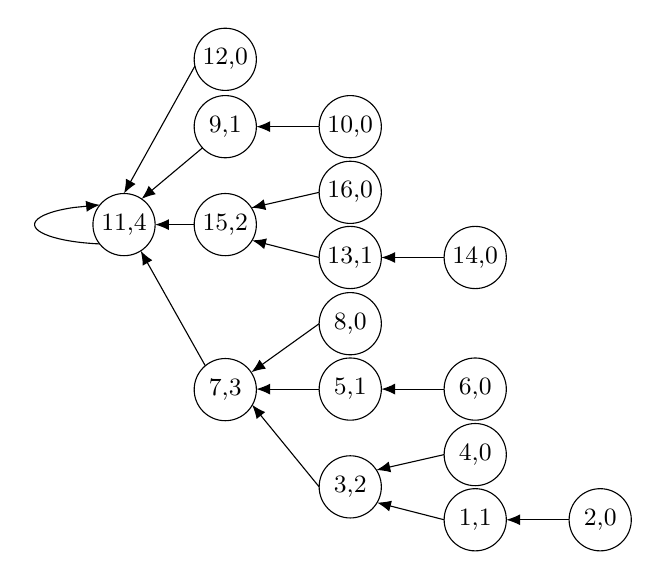
\begin{tikzpicture}\small
\draw (2.8898,-3.3172) circle (0.3949cm); 
\node at (2.8898,-3.3172) {3,2};
\draw (4.4771,-2.0753) circle (0.3949cm); 
\node at (4.4771,-2.0753) {6,0};
\draw (1.3026,-2.0822) circle (0.3949cm); 
\node at (1.3026,-2.0822) {7,3};
\draw (2.8898,-1.2448) circle (0.3949cm); 
\node at (2.8898,-1.2448) {8,0};
\draw (4.4771,-3.7350) circle (0.3949cm); 
\node at (4.4771,-3.7350) {1,1};
\draw (6.0643,-3.7350) circle (0.3949cm); 
\node at (6.0643,-3.7350) {2,0};
\draw (2.8898,-2.0753) circle (0.3949cm); 
\node at  (2.8898,-2.0753)  {5,1};
\draw (4.4771,-2.9075) circle (0.3949cm); 
\node at (4.4771,-2.9075) {4,0};
\draw (2.8898,1.2573) circle (0.3949cm); 
\node at (2.8898,1.2573) {10,0};
\draw (1.3026,0.0135) circle (0.3949cm); 
\node at (1.3026,0.0135) {15,2};
\draw (0.0168,0.0135) circle (0.3949cm); 
\node at (0.0168,0.0135) {11,4};
\draw [arrows = {-Latex[width=0pt 10, length=5pt 0]}] (-0.2928,-0.2317)  arc [start angle=260, end angle=120,
x radius=1cm, y radius=2.5mm] -- (-0.2888,0.2638);
\draw (1.3026,1.2573) circle (0.3949cm); 
\node at (1.3026,1.2573) {9,1};
\draw (2.8898,-0.4042) circle (0.3949cm); 
\node at (2.8898,-0.4042) {13,1};
\draw (4.4771,-0.4042) circle (0.3949cm); 
\node at (4.4771,-0.4042) {14,0};
\draw (2.8898,0.4233) circle (0.3949cm); 
\node at (2.8898,0.4233) {16,0};
\draw (1.3026,2.1126) circle (0.3949cm); 
\node at (1.3026,2.1126) {12,0};
\draw[arrows = {-Latex[width=0pt 10, length=5pt]}] (4.0821,-2.0753)-- (3.2848,-2.0753);
\draw[arrows = {-Latex[width=0pt 10, length=5pt]}] (2.4949,-3.3172)-- (1.6434,-2.2750);
\draw[arrows = {-Latex[width=0pt 10, length=5pt]}] (2.4949,-1.2448)-- (1.6347,-1.8615);
\draw[arrows = {-Latex[width=0pt 10, length=5pt]}] (2.4949,-2.0753)-- (1.6976,-2.0753);
\draw[arrows = {-Latex[width=0pt 10, length=5pt]}] (5.6694,-3.7350)-- (4.8721,-3.7350);
\draw[arrows = {-Latex[width=0pt 10, length=5pt]}] (4.0821,-3.7350)-- (3.2306,-3.5169);
\draw[arrows = {-Latex[width=0pt 10, length=5pt]}] (4.0821,-2.9075)-- (3.2219,-3.1034);
\draw[arrows = {-Latex[width=0pt 10, length=5pt]}] (4.0821,-0.4042)-- (3.2848,-0.4042);
\draw[arrows = {-Latex[width=0pt 10, length=5pt]}] (0.9076,0.0135)-- (0.4117,0.0135);
\draw[arrows = {-Latex[width=0pt 10, length=5pt]}] (2.4949,1.2573)-- (1.6976,1.2573);
\draw[arrows = {-Latex[width=0pt 10, length=5pt]}] (1.0135,0.9882)-- (0.2397,0.3396);
\draw[arrows = {-Latex[width=0pt 10, length=5pt]}] (2.4949,0.4233)-- (1.6347,0.2273);
\draw[arrows = {-Latex[width=0pt 10, length=5pt]}] (2.4949,-0.4042)-- (1.6434,-0.1861);
\draw[arrows = {-Latex[width=0pt 10, length=5pt]}] (0.9170,2.0271)-- (0.0168,0.4085);
\draw[arrows = {-Latex[width=0pt 10, length=5pt]}] (1.0490,-1.7794)--(0.2288,-0.3197);
\end{tikzpicture}


3.

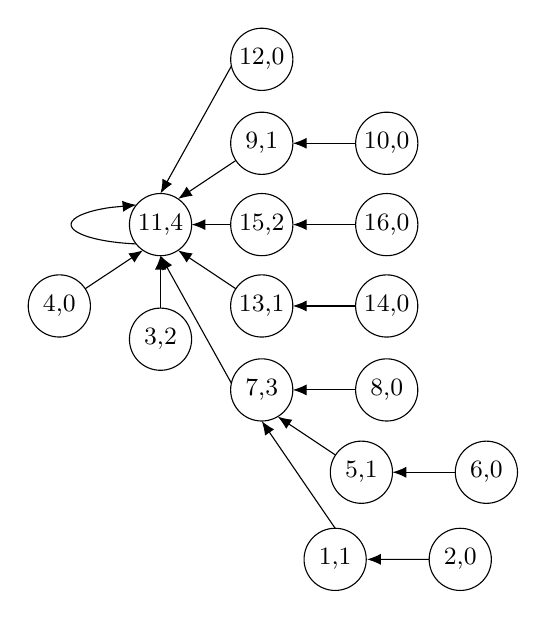
\begin{tikzpicture}\small
\draw (2.5681,-3.1314) circle (0.3949cm); 
\node at (2.5681,-3.1314) {5,1};
\draw (4.1553,-3.1316) circle (0.3949cm); 
\node at (4.1553,-3.1316) {6,0};
\draw (2.8893,-1.0198) circle (0.3949cm); 
\node at (2.8893,-1.0198) {14,0};
\draw (2.8893,-2.0861) circle (0.3949cm); 
\node at (2.8893,-2.0861) {8,0};
\draw (3.8234,-4.2380) circle (0.3949cm); 
\node at (3.8234,-4.2380) {2,0};
\draw (-1.2685,-1.0196) circle (0.3949cm); 
\node at (-1.2685,-1.0196) {4,0};
\draw (0.0168,-1.4419) circle (0.3949cm); 
\node at (0.0168,-1.4419) {3,2};
\draw (2.2345,-4.2378) circle (0.3949cm); 
\node at  (2.2345,-4.2378) {1,1};
\draw (1.3026,0.0135) circle (0.3949cm); 
\node at (1.3026,0.0135) {15,2};
\draw (1.3026,2.1126) circle (0.3949cm); 
\node at (1.3026,2.1126) {12,0};
\draw (0.0168,0.0135) circle (0.3949cm); 
\node at (0.0168,0.0135) {11,4};
\draw [arrows = {-Latex[width=0pt 10, length=5pt 0]}] (-0.2928,-0.2317)  arc [start angle=260, end angle=120,
x radius=1cm, y radius=2.5mm] -- (-0.2888,0.2638);
\draw (1.3026,1.0463) circle (0.3949cm); 
\node at (1.3026,1.0463) {9,1};
\draw (2.8898,1.0463) circle (0.3949cm); 
\node at (2.8898,1.0463) {10,0};
\draw (2.8898,0.0135) circle (0.3949cm); 
\node at (2.8898,0.0135) {16,0};
\draw (1.3021,-1.0196) circle (0.3949cm); 
\node at (1.3021,-1.0196) {13,1};
\draw (1.3021,-2.0859) circle (0.3949cm); 
\node at  (1.3021,-2.0859) {7,3};
\draw[arrows = {-Latex[width=0pt 10, length=5pt]}] (3.7603,-3.1316)-- (2.9630,-3.1316);
\draw[arrows = {-Latex[width=0pt 10, length=5pt]}] (2.2392,-2.9127)-- (1.5051,-2.4246);
\draw[arrows = {-Latex[width=0pt 10, length=5pt]}] (2.4943,-2.0861)-- (1.6970,-2.0861);
\draw[arrows = {-Latex[width=0pt 10, length=5pt]}] (-0.9396,-0.8009)-- (-0.2056,-0.3129);
\draw[arrows = {-Latex[width=0pt 10, length=5pt]}] (0.0168,-1.0469)-- (0.0168,-0.3814);
\draw[arrows = {-Latex[width=0pt 10, length=5pt]}] (2.4943,-1.0198)-- (1.6970,-1.0198);
\draw[arrows = {-Latex[width=0pt 10, length=5pt]}] (0.9170,2.0271)-- (0.0168,0.4085);
\draw[arrows = {-Latex[width=0pt 10, length=5pt]}] (0.9076,0.0135)-- (0.4117,0.0135);
\draw[arrows = {-Latex[width=0pt 10, length=5pt]}] (0.9737,0.8276)-- (0.2397,0.3396);
\draw[arrows = {-Latex[width=0pt 10, length=5pt]}] (0.9731,-0.8009)-- (0.2391,-0.3129);
\draw[arrows = {-Latex[width=0pt 10, length=5pt]}] (2.4949,0.0135)-- (1.6976,0.0135);
\draw[arrows = {-Latex[width=0pt 10, length=5pt]}] (2.4949,1.0463)-- (1.6976,1.0463);
\draw[arrows = {-Latex[width=0pt 10, length=5pt]}] (0.9164,-2.0004)--(0.0168,-0.3814);
\draw[arrows = {-Latex[width=0pt 10, length=5pt]}] (2.2345,-3.8428)--(1.3021,-2.4809);
\draw[arrows = {-Latex[width=0pt 10, length=5pt]}] (3.4284,-4.2380)--(2.6395,-4.2378);
\end{tikzpicture}

\newpage
$\text{Q}_{2}$

a.

1.

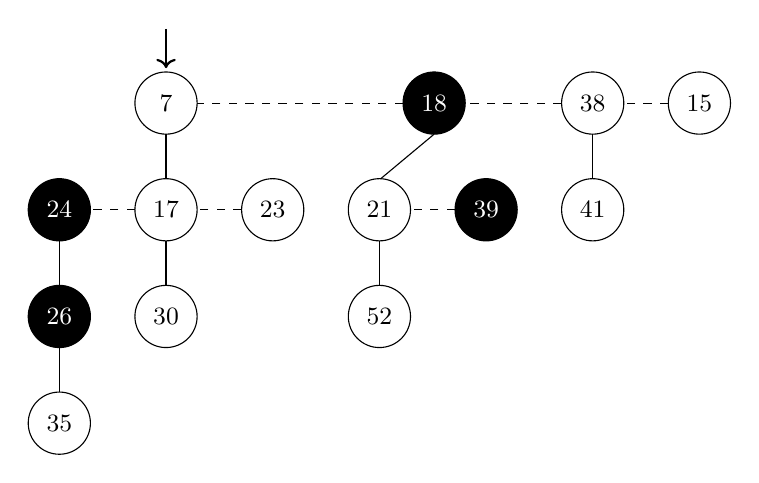
\begin{tikzpicture}\small
\draw[fill=black, draw=black] (2.6103,-0.0985) circle (0.3949cm); 
\node[text=mytextcolor] at (2.6103,-0.0985) {39};
\draw (-2.8100,-2.8086) circle (0.3949cm); 
\node at (-2.8100,-2.8086) {35};
\draw[fill=black, draw=black]  (-2.8100,-1.4536) circle (0.3949cm); 
\node[text=mytextcolor]  at (-2.8100,-1.4536) {26};
\draw (3.9640,1.2566) circle (0.3949cm); 
\node at (3.9640,1.2566) {38};
\draw (1.2552,-1.4536) circle (0.3949cm); 
\node at (1.2552,-1.4536) {52};
\draw (5.3191,1.2566) circle (0.3949cm); 
\node at (5.3191,1.2566) {15};
\draw (3.9640,-0.0985) circle (0.3949cm); 
\node at (3.9640,-0.0985) {41};
\draw (-1.4549,-0.0985) circle (0.3949cm); 
\node at (-1.4549,-0.0985) {17};
\draw[fill=black, draw=black] (1.9501,1.2566) circle (0.3949cm); 
\node[text=mytextcolor] at (1.9501,1.2566) {18};
\draw (-1.4549,1.2566) circle (0.3949cm); 
\node at (-1.4549,1.2566) {7};
\draw (-0.0998,-0.0985) circle (0.3949cm); 
\node at (-0.0998,-0.0985) {23};
\draw (-1.4549,-1.4536) circle (0.3949cm); 
\node at (-1.4549,-1.4536) {30};
\draw[fill=black, draw=black] (-2.8100,-0.0985) circle (0.3949cm); 
\node[text=mytextcolor]  at (-2.8100,-0.0985) {24};
\draw (1.2552,-0.0985) circle (0.3949cm); 
\node at (1.2552,-0.0985) {21};
\draw  (3.9640,0.2965)-- (3.9640,0.8616);
\draw[dashed]  (2.2154,-0.0985)-- (1.6502,-0.0985);
\draw  (1.2725,0.2965)-- (1.9501,0.8616);
\draw[dashed]  (4.9242,1.2566)-- (4.3590,1.2566); 
\draw  (1.2552,-1.0586)-- (1.2552,-0.4934);
\draw[dashed]  (3.5691,1.2566)-- (2.3450,1.2566);
\draw  (-2.8100,-2.4137)-- (-2.8100,-1.8485);
\draw[dashed]  (-0.4948,-0.0985)-- (-1.0599,-0.0985);
\draw  (-1.4549,0.2965)-- (-1.4549,0.8616);
\draw[dashed]  (1.5551,1.2566)-- (-1.0599,1.2566);
\draw  (-2.8100,-1.0586)-- (-2.8100,-0.4934);
\draw  (-1.4549,-1.0586)-- (-1.4549,-0.4934);
\draw[dashed]  (-1.8499,-0.0985) -- (-2.4150,-0.0985);
\draw[->, thick] (-1.4549,2.2) -- (-1.4549,1.7);
\end{tikzpicture}
\vspace{1cm}

2.

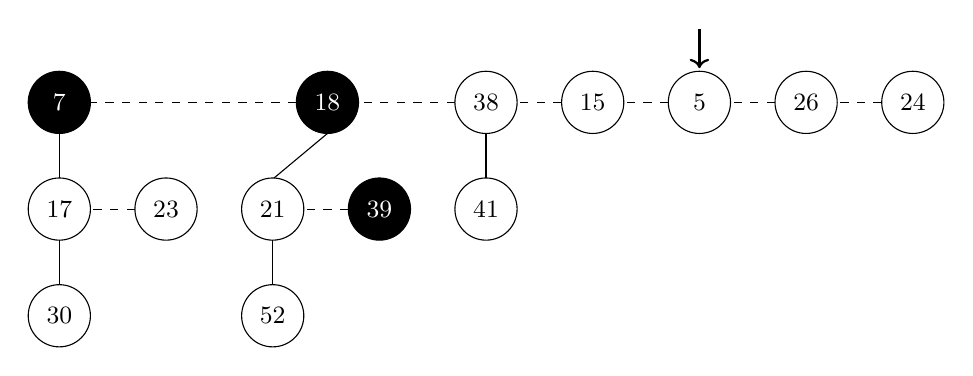
\begin{tikzpicture}\small
\draw (-0.5727,-2.3447) circle (0.3949cm); 
\node at (-0.5727,-2.3447) {52};
\draw (2.1361,-0.9897) circle (0.3949cm); 
\node at (2.1361,-0.9897) {41};
\draw (2.1361,0.3654) circle (0.3949cm); 
\node at (2.1361,0.3654) {38};
\draw (3.4912,0.3654) circle (0.3949cm); 
\node at (3.4912,0.3654) {15};
\draw (7.5564,0.3654) circle (0.3949cm); 
\node at (7.5564,0.3654) {24};
\draw (6.2013,0.3654) circle (0.3949cm); 
\node at (6.2013,0.3654) {26};
\draw (4.8462,0.3654) circle (0.3949cm); 
\node at (4.8462,0.3654) {5};
\draw (-3.2829,-0.9897) circle (0.3949cm); 
\node at (-3.2829,-0.9897) {17};
\draw[fill=black, draw=black] (0.1221,0.3654) circle (0.3949cm); 
\node[text=mytextcolor] at (0.1221,0.3654) {18};
\draw[fill=black, draw=black] (-3.2829,0.3654) circle (0.3949cm); 
\node[text=mytextcolor] at (-3.2829,0.3654) {7};
\draw (-1.9278,-0.9897) circle (0.3949cm); 
\node at (-1.9278,-0.9897) {23};
\draw[fill=black, draw=black] (0.7824,-0.9897) circle (0.3949cm); 
\node[text=mytextcolor] at (0.7824,-0.9897) {39};
\draw (-3.2829,-2.3447) circle (0.3949cm); 
\node at (-3.2829,-2.3447) {30};
\draw (-0.5727,-0.9897) circle (0.3949cm); 
\node at (-0.5727,-0.9897) {21};
\draw[dashed]  (3.0962,0.3654)-- (2.5311,0.3654);
\draw  (-0.5727,-1.9498)-- (-0.5727,-1.3846);
\draw[dashed]  (1.7411,0.3654)-- (0.5171,0.3654);
\draw[dashed]  (7.1614,0.3654)-- (6.5963,0.3654);
\draw[dashed]  (5.8063,0.3654)-- (5.2412,0.3654);
\draw[dashed]  (4.4513,0.3654)-- (3.8861,0.3654);
\draw  (2.1361,-0.5947)-- (2.1361,-0.0296);
\draw[dashed]  (-2.3227,-0.9897)-- (-2.8879,-0.9897);
\draw  (-3.2829,-0.5947)-- (-3.2829,-0.0296);
\draw[dashed]  (-0.2729,0.3654)-- (-2.8879,0.3654);
\draw[dashed]  (0.3874,-0.9897)-- (-0.1777,-0.9897);
\draw  (-0.5554,-0.5947)-- (0.1221,-0.0296);
\draw  (-3.2829,-1.9498) -- (-3.2829,-1.3846);
\draw[->, thick] (4.8462, 1.3) -- (4.8462, 0.8);
\end{tikzpicture}
\vspace{1cm}

3.

Final one

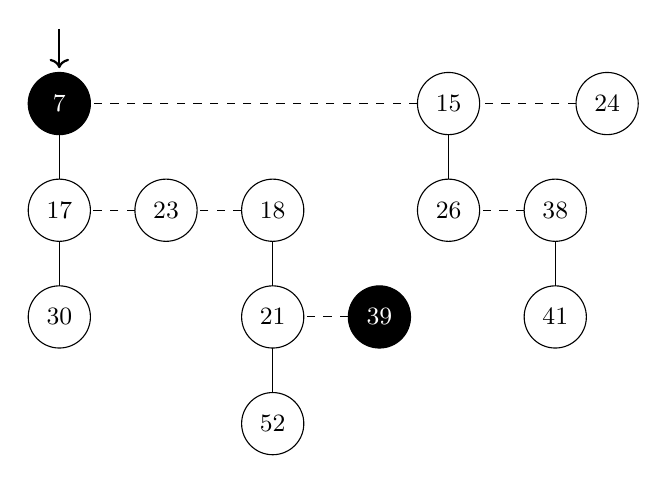
\begin{tikzpicture}\small
\draw (4.8945,1.5505) circle (0.3949cm); 
\node at (4.8945,1.5505) {24};
 \draw (0.6473,-1.1596) circle (0.3949cm); 
\node at (0.6473,-1.1596) {21};
 \draw (2.8805,0.1955) circle (0.3949cm); 
\node at (2.8805,0.1955) {26};
 \draw (4.2356,-1.1596) circle (0.3949cm); 
\node at (4.2356,-1.1596) {41};
 \draw (4.2356,0.1955) circle (0.3949cm); 
\node at (4.2356,0.1955) {38};
 \draw (0.6473,-2.5147) circle (0.3949cm); 
\node at (0.6473,-2.5147) {52};
 \draw (2.8805,1.5505) circle (0.3949cm); 
\node at (2.8805,1.5505) {15};
 \draw (-0.7077,0.1955) circle (0.3949cm); 
\node at (-0.7077,0.1955) {23};
 \draw (-2.0628,0.1955) circle (0.3949cm); 
\node at (-2.0628,0.1955) {17};
\draw[fill=black, draw=black] (-2.0628,1.5505) circle (0.3949cm); 
\node[text=mytextcolor] at (-2.0628,1.5505) {7};
 \draw[fill=black, draw=black] (2.0024,-1.1596) circle (0.3949cm); 
\node[text=mytextcolor] at (2.0024,-1.1596) {39};
 \draw (-2.0628,-1.1596) circle (0.3949cm); 
\node at (-2.0628,-1.1596) {30};
 \draw (0.6473,0.1955) circle (0.3949cm); 
\node at (0.6473,0.1955) {18};
\draw  (0.6473,-2.1197)-- (0.6473,-1.5546);
\draw[dashed]  (0.2524,0.1955)-- (-0.3128,0.1955);
\draw  (0.6473,-0.7646)-- (0.6473,-0.1995); 
\draw[dashed]  (4.4995,1.5505)-- (3.2755,1.5505);
\draw[dashed]  (3.8406,0.1955)-- (3.2755,0.1955);
\draw  (4.2356,-0.7646)-- (4.2356,-0.1995);
\draw[dashed]  (-1.1027,0.1955)-- (-1.6678,0.1955);
\draw  (-2.0628,0.5904)-- (-2.0628,1.1556);
\draw[dashed]  (2.4856,1.5505)-- (-1.6678,1.5505);
\draw  (2.8805,0.5904)-- (2.8805,1.1556);
\draw[dashed]  (1.6074,-1.1596)-- (1.0423,-1.1596);
\draw  (-2.0628,-0.7646) --  (-2.0628,-0.1995);
\draw[->, thick] (-2.0628, 2.5) -- (-2.0628, 2.0);
\end{tikzpicture}



 A[0]={\small\textcircled{\scriptsize{24}}}
 
  A[1]=nil 
  
   A[2]= {\small\textcircled{\scriptsize{15}}} 
   
   A[3]={\small\textcircled{\scriptsize{7}}}


b. 

decrease-priority({\small\textcircled{\scriptsize{38}}},8)

decrease-priority({\small\textcircled{\scriptsize{21}}},6)

extract-min()

\newpage
$\text{Q}_{3}$

1.

Suppose capacity $=$ size $=m$

we first use $m / 2$ times of remove ()

Then after we execute the $m / 2$ time remove (), size $=m / 2=\frac{1}{2}$ capacity.

$\Rightarrow$ We create a new array with capacity $=m / 2$ and copy all the remaining $m / 2$ elements of the old array into the new array.

$\Rightarrow$ time complexity : $\Omega(m / 2)$

Now we use add() one time, as size $=$ capacity $=m / 2$ 

we need to double the array and copy all the $m / 2$ elements

$\Rightarrow$ time complexity, $\Omega(m / 2)$

At this time, 

size $=m / 2+1 \quad$

capacity $=m$

We use remove() again.

After removing the last one, size $=m / 2$, capacity $=m$, so we need a new shorter array again and copy all the $m / 2$ elements.

$\Rightarrow$ time complexity $=\Omega(m / 2)$

Consider the combo: add() + remove(), it can maintain the size and capacity be $m / 2$

So after executing remove() $m / 2$ times, we can run the combo: add() + remove() for the remaining $3 m-m / 2=\frac{5}{2} m$ operations:

$\Rightarrow$ We can run the combo $\frac{5}{2} m \times \frac{1}{2}=\frac{5}{4} m$ times.

Each combo has complexity $\Omega(m / 2)+\Omega(m / 2)=\Omega(m)$ $\Rightarrow$ the total time complexity is $\Omega\left(m^2\right)$, as wanted.

$\therefore 3 m$ operations are: {\small\textcircled{\scriptsize{1}}} remove() $\times m / 2 $ 
 {\small\textcircled{\scriptsize{2}}} (add()+ remove()) $\times \frac{5}{4} \mathrm{~m}$

\newpage

2.

add(): receive $\$ 7$. spend $\left\{\begin{array}{l}\text { if copying: } \$ \text { capacity }+1 \text { (use ``capacity'' before add) } \\ \text { if no copying: } \$ 1\end{array}\right.$ 

remove(): receive $\$ 4$, spend $\left\{\begin{array}{l}\text { if copying } \$ \text { size }-1 \text { (use ``size'' before remove) } \\ \text { if no copying: } \$ 1\end{array}\right.$

Prove Invariant: amount $\geq$ capacity-size.

Initially: amount $=0=$ capacity-size.

remove:

Assume the size before remove is $s$

Assume the capacity before remove is $c$

Assume the amount $=a \geqslant c-s$ before remove

if copying:


$ a^{\prime}=a+4-(s-1)=a-s+3 $

$ c^{\prime}=\frac{1}{2} c $

$ s^{\prime}=s-1$


$s-1 \leq \frac{1}{4} c$ by remove algorithm

$ c^{\prime}-s^{\prime}=\frac{1}{2} c-s+1 $

$ \therefore a^{\prime}-\left(c^{\prime}-s^{\prime}\right)=a-s+3-\left(\frac{1}{2} c-s+1\right)=a-\frac{1}{2} c+2 \geqslant c-s-\frac{1}{2} c+2=\frac{1}{2} c-s+2\geqslant \frac{1}{2} c-2 s+2(\text{by } s \ge 0 \text{ in given invariant} ) $

$ \because s-1 \leq \frac{1}{4} c \Rightarrow \frac{1}{2} c-2 s+2 \geqslant 0 \Rightarrow a^{\prime}-\left(c^{\prime}-s^{\prime}\right) \geqslant \frac{1}{2} c-2 s+2 \geqslant 0 $

$ \Rightarrow a^{\prime} \geqslant c^{\prime}-s^{\prime}$


$2^{\circ}$ if no copying

$ a^{\prime}=a+4-1=a+3 $

$ c^{\prime}=c $

$ s^{\prime}=s-1 $

$ a^{\prime}=a+3 \geqslant c-s+3>c-s+1=c-(s-1)=c^{\prime}-s^{\prime}$


add:

Assume the size before add is $s$

Assume the capacity before add is $c$

Assume the amount $=a \geqslant c-s$ before add

if copying:

$ a^{\prime}=a+3-(c+1) $

$ c^{\prime}=2 c $

$ s^{\prime}=s+1 $

$ c^{\prime}-s^{\prime}=2 c-s-1 $

$ a^{\prime}-\left(c^{\prime}-s^{\prime}\right)=a+2-c-(2 c-s-1)=a+2-3 c+s+1  =a-3 c+3+s$


Since last copying, no matter whether the last copying is from remove or add, $c / 2$ cells have $\$ 6$ saved each.

$\Rightarrow$ total saved $\$ c / 2 \cdot 6=3 c$

As amount after last copying is amount $\geqslant$ capacity-size $\geqslant 0$,
$ a \geqslant 3 c $

$ \Rightarrow a^{\prime}-\left(c^{\prime}-s^{\prime}\right)=a-3 c+3+5 \geqslant 0$

$\Rightarrow a^{\prime} \geqslant c^{\prime}-s^{\prime}$

if no copying:

$ a^{\prime}=a+7-1=a+6 $

$ c^{\prime}=c $

$ s^{\prime}=s+1 $

$ a^{\prime}=a+6 \geqslant c-s+6>c-s-1=c-(s+1)=c^{\prime}-s^{\prime} $

$ \Rightarrow a^{\prime} \geqslant c^{\prime}-s^{\prime}$



By 4 cases mentioned above,

$a^{\prime} \geqslant c^{\prime}-s^{\prime} \geqslant 0$

$\therefore$ add and remove each take $O(7)$ and $O(4)$ amortized time

$\because O(7)=O(4)=O(1)$

$\therefore$ add and remove each take $O(1)$ amortized time.

\newpage
$\text{Q}_{4}$

1. t-delete worst-case time: $\Theta(s \operatorname{logs})$

2. PF :

$\text {t-insert }(x): O(\lg s)( s \geqslant c / 2 \Rightarrow 2 s \geqslant c \Rightarrow\lg c \leq \lg (2 s) \in O(\lg (s)) \Rightarrow O(\lg (c)) \subseteq O(\lg (s))) $

$ \text {t-search }(x)=O(\lg s)( s \geqslant c / 2 \Rightarrow 2 s \geqslant c \Rightarrow\lg c \leqslant \lg (2 s) \in O(\lg (s)) \Rightarrow O(\lg (c)) \subseteq O(\lg (s))) $

$\text {t-delete }(x): O(s \lg s)(c+s \lg s \leq 2 s+s \lg (s) \in O(s \lg (s)) \Rightarrow O(c+s \lg s) \subseteq O(s \lg (s)))$



Define potential function: $\Phi(T)=c+(c-s) \operatorname{\lg s}$

WTP: $\Phi\left(T_i\right) \geqslant 0 \quad \forall i \in N$

Initially: $\Phi\left(T_0\right)=0+(0-0) \lg 0=0$

Assume $\Phi\left(T_{i-1}\right) \geqslant 0$

t-insert:

If found used, no change to $c$ and s.

$\Rightarrow \Phi\left(T_i\right)=\Phi\left(T_{i-1}\right) \geqslant 0$

If found unused:

$ c_i=c_{i-1} $

$ s_i=s_{i-1}+1 $

$ \because c_i \geqslant s_i $

$ \therefore c_{i-1} \geqslant s_{i-1}+1 $

$ \Phi\left(T_i\right)= c_i+\left(c_i-s_i\right)\lg (s_i)=\underset{\geqslant 0}{ c_{i-1}}+\left(c_{i-1}-\underset{\geqslant 0}{ s_{i-1}}-1\right)  
\lg\left(\underset{\geqslant 0}{ s_{i-1}}+1\right) \geqslant 0
$


If not found:

$c_i=c_{i-1}+1$

$s_i=s_{i-1}+1$

$\Phi\left(T_i\right)=c_i+\left(c_i-s_i\right)\lg (s_i)=\underset{\geqslant 0}{c_{i-1}+1}+\underset{\geqslant 0}{\left(c_{i-1}+1-s_{i-1}-1\right)}\lg\underset{\geqslant 0}{\left(s_{i-1}+1\right)} \geqslant 0$

t-search:

no change to $c$ and s, $\Rightarrow \Phi\left(T_i\right)=\Phi\left(T_{i n}\right) \geqslant 0$ 

t-delete:

If not found:

no change to $c$ and $s \Rightarrow \Phi\left(T_i\right)=\Phi\left(T_{i-1}\right) \geq 0$ 

If found without creating new AVL:

$ c_i=c_{i-1} $

$ s_i=s_{i-1}-1 $

$ \Phi\left(T_i\right)=c_i+\left(c_{i}-s_i\right) \lg \left(s_i\right)=c_{i-1}+\left(c_{i-1}-s_{i-1}+1\right)\lg\left(s_{i-1}-1\right) $

$ \because s_i \geqslant c_i / 2  $ by invariant

$ \Rightarrow s_{i-1}-1 \geqslant c_{i-1} / 2 $

If  $  s_{i-1}=0$, we have $0-1 \geqslant c_{i-1} / 2$.

$\Rightarrow-2 \geqslant c_{i-1} $

But $c_{i-1} \geqslant 0$.

$ \Rightarrow$ contradiction

$ \Rightarrow s_{i-1} \neq 0 $

If  $  s_{i-1}=1$, we have $0 \geqslant c_{i-1} / 2$.

$\because c_{i-1} \geqslant 0$

$\therefore c_{i-1}=0<s_{i-1} \Rightarrow $ impossible

$ \therefore s_{i-1}\ne 1 $

$ \because s_{i-1} \geqslant 0 $

$ \therefore s_{i-1} \geqslant 2 $

$ \therefore s_{i-1}-1 \geqslant 1 \Rightarrow \lg \left(s_{i-1}-1\right) \geqslant 0 $

$ \therefore \Phi\left(T_i\right)=\underset{\geqslant 0}{c_{i-1}}+\underset{\geqslant 0}{\left(c_{i-1}-s_{i-1}+1\right)}\lg\underset{\geqslant 0}{\left(s_{i-1}-1\right)} \geqslant 0$

If found and creating new AVL:

$ c_i=s_i $

$\Rightarrow  \Phi\left(T_i\right)=c_i \geqslant 0$



By the cases mentioned above,

$ \Phi\left(T_i\right) \geqslant 0, \forall i \in  N $

$ \because \Phi\left(T_0\right)=0 $

$ \therefore \Phi\left(T_n\right)-\Phi\left(T_0\right)=\Phi\left(T_n\right)-0 \geqslant 0, \forall n \geqslant 0$


t-insert:

If not found:

$\begin{aligned}
   \Delta ( \Phi)&=\Phi\left(T_i\right)-\Phi\left(T_{i-1}\right) \\
  & =c_i+\left(c_{i}-s_i\right) \lg \left(s_i\right)-\left(c_{i-1}+\left(c_{i-1}-s_{i-1}\right) \lg \left(s_{i-1}\right)\right)\\
& =c_{i-1}+1+\left(c_{i-1}+1-s_{i-1}-1\right) \lg \left(s_{i-1}+1\right)-\left(c_{i-1}+\left(c_{i-1}-s_{i-1}\right) \lg \left(s_{i-1}\right)\right) \\
& =1+\left(c_{i-1}-s_{i-1}\right)\left(\lg \left(s_{i-1}+1\right)-\lg \left(s_{i-1}\right)\right) \\
&=1+\left(c_{i-1}-s_{i-1}\right)\left(\lg \left(1+\frac{1}{s_{i-1}}\right)\right)  
\end{aligned}  $



$ \because(1+1 / k)^k \leq e $

$ \therefore \ln (1+1 / k)^k \leq 1 $

$ \therefore \ln (1+1 / k) \leq \frac{1}{k} $

$ \therefore \lg (1+1 / k)=\frac{\ln (1+1 / k)}{\ln 2} \leq \frac{1}{(\ln2) k} (\#)$

$ \Rightarrow \Delta(\Phi)=1+\left(c_{i-1}-s_{i-1}\right)\left(\lg\left(1+\frac{1}{s_{i-1}}\right)\right) $

$ \leq 1+\frac{1}{l_{n 2}} \cdot \frac{c_{i-1}-s_{i-1}}{s_{i-1}} $

$ \because s_{i-1} \geqslant c_{i-1} / 2  $ by invariant

$ \therefore \frac{c_{i-1}-s_{i-1}}{s_{i-1}}=\frac{c_{i-1}}{s_{i-1}}-1 \leq 2-1=1 (\triangle)$

$ \Rightarrow \Delta(\Phi) \leq 1+\frac{1}{ \ln 2} $

$ \therefore a_i=t_i+\Delta(\Phi) \leq \lg \left(s_i\right)+1+\frac{1}{\ln 2} \in O (\lg (s_i)) $ 

$\therefore$ In this case, t-insert operation takes amortized time  $O (\lg s) $ 

If found unused:

$\begin{aligned}
   \Delta(\Phi)  &=\Phi\left(T_i\right)-\Phi\left(T_{i-1}\right) \\ 
& =c_i+\left(c_{i}-s_i\right) \lg \left(s_i\right)-\left(c_{i-1}+\left(c_{i-1}-s_{i-1}\right) \lg \left(s_{i-1}\right)\right) \\
& =c_{i-1}+\left(c_{i-1}-s_{i-1}-1\right) \lg \left(s_{i-1}+1\right)-c_{i-1}-\left(c_{i-1}-s_{i-1}\right) \lg \left(s_{i-1}\right) \\
& =\left(c_{i-1}-s_{i-1}\right)\left(\lg \left(s_{i-1}+1\right)-\lg \left(s_{i-1}\right)\right)-\lg \left(s_{i-1}+1\right) 
\\
& \leq\left(c_{i-1}-s_{i-1}\right)\left(\lg \left(1+\frac{1}{s_{i-1}}\right)\right) (\because \lg \left(s_{i-1}+1\right) \geq 0 )\\
& \leq\left(c_{i-1}-s_{i-1}\right)\left(\frac{1}{(\ln 2) s_{i-1}}\right) \text{ by(\#)}\\
& =\frac{1}{\ln 2}\left(\frac{c_{i-1}-s_{i-1}}{s_{i-1}}\right) \\ &\leq \frac{1}{\ln 2}  \text{ by(}\triangle\text{)}
\end{aligned} $



$\Rightarrow a_i \leqslant \lg \left(s_i\right)+\frac{1}{\ln 2} \in O\left(\lg \left(s_i\right)\right)$

$\therefore $ In this case, t-insert operation takes amortized time $O(\lg s)$

If found used:

no change to $c$ and $s$

$ \Rightarrow \Delta(\Phi)=0 $

$ \therefore a_i=\lg \left(s_i\right)+0=\lg \left(s_i\right) \in O\left(\lg \left(s_i\right)\right)$


$\therefore$ In this case, t-insert operation takes amortized time $O(\lg s)$

t-search:

No change to $c$ and $s$.

$ \Rightarrow \Delta (\Phi)=0 $

$ \therefore a_i=\lg \left(s_i\right)+0=\lg \left(s_i\right) \in O\left(\lg \left(s_i\right)\right)$


$\therefore$ In this case, t-search operation takes amortized time $O(\lg s)$

t-delete:

If found and creating a new AVL:

$\begin{aligned}
  \Delta(\Phi) & =c_i+\left(c_i-s_i\right)\lg\left( s_i\right)-c_{i-1}-\left(c_{i-1}-s_{i-1}\right) \lg \left(s_{i-1}\right)\\
  &=\left(s_{i-1}-1\right)+0-c_{i-1}-\left(c_{i-1}-s_{i-1}\right) \lg \left(s_{i-1}\right)
\end{aligned} $

$\because s_{i-1}-1<c_{i-1} / 2$ (the condition to creat a new AVL)

$\therefore 2 s_{i-1}-2  < c_{i-1}$

$\begin{aligned}\therefore \Delta(\Phi) & <\left(s_{i-1}-1\right)-\left(2 s_{i-1}-2\right)-\left(2 s_{i-1}-2-s_{i-1}\right) \lg \left(s_{i-1}\right) \\
& =-\left(s_{i-1}-1\right)-\left(s_{i-1}-2\right) \lg \left(s_{i-1}\right)
\end{aligned} $


$\begin{aligned}a_{i}&=t_i+\Delta(\Phi)\\
& <s_i \lg \left(s_i\right)-\left(s_{i-1}-1\right)-\left(s_{i-1}-2\right) \lg \left(s_{i-1}\right) \\
& =\left(s_{i-1}-1\right) \lg \left(s_{i-1}-1\right)-\left(s_{i-1}-1\right)-\left(s_{i-1}-1\right) \lg \left(s_{i-1}\right)+\lg \left(s_{i-1}\right) \\
&=\left(s_{i-1}-1\right)\left(\lg \left(s_{i-1}-1\right)-\lg \left(s_{i-1}\right)-1\right)+\lg \left(s_{i-1}\right) \\
& =\left(s_{i-1}-1\right)\left(\lg \left(\frac{s_{i-1}-1}{s_{i-1}}\right)-1\right)+\lg\left(s_{i-1}\right)\quad(s_{i-1} \geq 1 \text{ as need at least 1 node to be deleted)}\\
& <\left(s_{i-1}-1\right)\left(\lg \left(\frac{s_{i-1}+1}{s_{i-1}}\right)-1\right)+\lg\left(s_{i-1}\right)\quad \text {( by } y=\lg (x) \text{is monotonically increasing)} \\
& <\left(s_{i-1}-1\right)\left(\frac{1}{(\ln 2)s_{i-1}}-1\right)+\lg \left(s_{i-1}\right)\text {(by } (\#)\text {)} \\
&=\frac{1}{\ln2}-\frac{1}{(\ln 2)s_{i-1})}-s_{i-1}+1+\lg \left(s_{i-1}\right)\\
&<1+\frac{1}{\ln 2}+\lg \left(s_{i}+1\right) \in O\left(\lg \left(s_{i}\right)\right)
\end{aligned} $


$\therefore $ In this case, t-delete operation takes amortized time $O(\lg s)$.

If found but no copying:


$\begin{aligned}\Delta(\Phi) & =c_i+\left(c_i-s_i\right)\lg\left(s_i\right)-c_{i-1}-\left(c_{i-1}-s_{i-1}\right) \lg \left(s_{i-1}\right) \\
&=c_{i-1}+\left(c_{i-1}-s_{i-1}+1\right) \lg \left(s_{i-1}-1\right)-c_{i-1}-\left(c_{i-1}-s_{i-1}\right) \lg \left(s_{i-1}\right) \\
&=\left(c_{i-1}-s_{i-1}\right)\left(\lg \left(s_{i-1}-1\right)-\lg \left(s_{i-1}\right)\right)+\lg \left(s_{i-1}-1\right) \\
& =\left(c_{i-1}-s_{i-1}\right)\left(\lg \left(\frac{s_{i-1}-1}{s_{i-1}}\right)\right)+\lg \left(s_i\right) \\
& <\left(c_{i-1}-s_{i-1}\right)\left(\lg\left(\frac{s_{i-1}+1}{s_{i-1}}\right)\right)+\lg \left(s_i\right) \\
& <\left(c_{i-1}-s_{i-1}\right) \cdot\left(\frac{1}{(\ln2)s_{i-1}}\right)+\lg \left(s_i\right) \text{(by } (\#) \text{) }\\
&\leqslant \frac{1}{\ln 2}+\lg \left(s_i\right) \text{(by } (\triangle) \text{)}
\end{aligned} $


$\begin{aligned}\therefore a_i & =t_i+\Delta(\Phi) \\
& =\lg \left(s_i\right)+\Delta(\Phi) \\
&\leqslant \frac{1}{\ln2}+\lg \left(s_i\right)+\lg \left(s_i\right) \in O\left(\lg \left(s_i\right)\right)
\end{aligned} $

$\therefore $  In this case, t-delete operation takes amortized time $O(\lg s)$ 

If not found:

No change to $c$ and $s$.

$ \Rightarrow \Delta(\Phi)=0 $

$ \therefore a_i=0+\lg\left(s_i\right) \in O\left(\lg \left(s_i\right)\right)$


$\therefore$ In this case, t-delete operation takes amortized time $O(\lg s)$

$\therefore$ Based on the cases mentioned above, each operation takes amortized time in $O(\lg s)$

QED.

\newpage
$\text{Q}_{5}$

1. $A_i=\sum\limits_{1\le j\le  n, j\ne i} B_{i, j}$

2. $E\left(B_{i, j}\right)= Pr\left(z_j\right.$ be the ancestor of $\left.z_i\right)$

Consider the key array $\left[z_{\min(i,j)}, z_{\max(i,j)}\right]$:

$z_{\min(i,j)}<z_{\min(i,j)+1} \ldots<x<\cdots<z_{\max(i ,j) }$

$1^{\circ}$ If $x$ is the first one to be picked from this array, then $z_{\min(i,j)}<x<z_{\max(i,j)}$. 

$\therefore z_i$ and $z_j$ will be separated two sides and $z_j$ can never be the ancestor of $z_i$.

$2^{\circ}$ If $z_i$ is the first one to be picked from this array, then we have either $z_j>z_i$ or $z_i>z_j$, but $z_j$ can't be the ancestor of $z_i$

$3^{\circ}$ If $z_j$ is the first one to be picked from this array:

If $z_i<z_j$, then $z_i$ will in $z_j$'s left sub-tree.

If $z_j<z_i$, then $z_i$ will in $z_j$'s right sub-tree.

In both cases, $z_j$ can be the ancestor of $z_i$.

$\begin{aligned}\therefore E\left(B_{i, j}\right)&= Pr\left(z_j \text { be the ancestor of } z_i\right)\\
&
= Pr\left(z_j\right.\text { is the first one to be picked in} \left[z_{\min(i, j)}, z_{\max( i, j)}\right])\\
&
=\frac{1}{|i-j|+1}
\end{aligned} $

3.

PF:

If $i \neq 1$ or $n \quad (i \in(1 , n)) $:

$\begin{aligned} E\left(A_i\right)&=E\left(\sum\limits_{j=1}^{i-1} B_{i, j}+\sum\limits_{j=i+1}^n B_{i, j}\right) \\
& =\sum\limits_{j=1}^{i-1} E\left(B_{i, j}\right)+\sum\limits_{j=i+1}^n E\left(B_{i, j}\right) \\
& =\sum\limits_{j=1}^{i-1} \frac{1}{|i-j|+1}+\sum\limits_{j=i +1 }^n \frac{1}{|i-j|+1} \\
& =\sum\limits_{k=2}^i \frac{1}{k}+\sum\limits_{k=2}^{n-i+1} \frac{1}{k}<2 \sum\limits_{k=1}^n \frac{1}{k}<2 \cdot \ln (n) \in O(\ln (n))
\end{aligned} $

If $i=1$:

$\begin{aligned}E(A_1)  &=E\left(\sum\limits_{j=2}^n B_{1, j}\right) \\
&=\sum\limits_{j=2}^n E(B_{1, j}) \\
& =\sum\limits_{j=2}^n \frac{1}{j} \\
& <\sum\limits_{j=1}^n \frac{1}{j}<\ln (n) \in O(\ln (n))
\end{aligned} $

If $i=n$:

$\begin{aligned}E\left(A_n\right)  &=E\left(\sum\limits_{j=1}^{n-1} B_{n, j}\right) \\
& =\sum\limits_{j=1}^{n-1} E\left(B_{n, j}\right) \\
& =\sum\limits_{j=1}^{n-1} \frac{1}{n-j+1} \\
&=\sum\limits_{k=2}^n \frac{1}{k}<\sum\limits_{k=1}^n \frac{1}{k}<\ln (n) \in O(\ln (n))
\end{aligned} $

By 3 cases mentioned above, $E\left(A_i\right) \in O(\ln (n))$.

QED.

\end{document}




